\section{Reproducing the experiments}\label{app:repro}

Each experiment lives in its own folder \texttt{experiments/E1}--\texttt{E4} of the repository, with one script, a README that documents the method in full, the input data and the saved results. The pinned versions highspy~1.15.1, networkx~3.6.1, NumPy~2.5.4 and SciPy~1.18.1 (\texttt{pip install -r requirements.txt}) are the recommended environment for reproducing all four. The saved results record their own environments: E1 ran with Python~3.12.14, NumPy~2.3.5 and SciPy~1.17.0 (whose bundled HiGHS is 1.8.0), E3 and E4 with highspy~1.15.1 and NumPy~2.4.1. A rerun of E1 with the pinned versions (SciPy's bundled HiGHS~1.12.0) on 12~November~2026 gave identical LP and ILP values, exactness, integrality, half-integral counts and LP iteration counts on all 1,012 instances; only B\&B node counts, which the report does not use, differed (on 114), apart from rounding-level differences in the B\&B dual bound. The rerun and a row-by-row comparison are saved in \texttt{experiments/E1/results/rerun-pinned-2026-11-12}. E4's README records the same agreement for its rerun. Timings differ between machines and runs. E2 additionally needs the CMR library~1.4.0, built from source (commit \texttt{0c42a44}; build steps in the E2 README), and its figures need Matplotlib (\texttt{requirements-analysis.txt}).

\begin{table}[H]
  \centering\footnotesize
  \caption{One command per experiment. Run times are from Apple~M-series laptops.}
  \label{tab:commands}
  \begin{tabular}{@{}lll@{}}
    \toprule
    & Command (run inside the experiment's folder) & Approximate run time \\
    \midrule
    E1 & \texttt{python3 e1.py} \quad (exhaustive self-test: \texttt{python3 e1.py -{}-check}) & 45\,s \\
    E2 & \texttt{python3 e2.py check -{}-with-cmr -{}-cmr PATH} & seconds \\
       & \texttt{python3 e2.py run -{}-cmr PATH -{}-time-limit 1 -{}-output results/NEW} & 20\,min \\
       & \texttt{python3 analyse.py results/main\_run -{}-plots} \quad (no recognition rerun) & seconds \\
    E3 & \texttt{python3 e3.py} & 1\,min \\
    E4 & \texttt{python3 e4.py} \quad (B\&B node check: \texttt{python3 e4.py -{}-node-check}) & 75\,s \\
    \bottomrule
  \end{tabular}
\end{table}

\paragraph{Solver settings.} Table~\ref{tab:settings} lists the settings that affect results. In E3, \emph{presolve} (a clean-up pass HiGHS runs before the main algorithm) is switched off. On graphs with a leaf $u$ attached to $v$, presolve fixes $x_u=0$ and $x_v=1$ by itself, which settles exactly the ties that E3 studies before simplex or IPM sees them. With presolve on, the experiment would partly measure presolve rather than the algorithms. E1 switches LP presolve off for the same reason, so that the reported vertex is the one simplex chose. No experiment sets a pivot rule, so HiGHS uses its defaults (\texttt{simplex\_dual\_edge\_weight\_strategy} and \texttt{simplex\_primal\_edge\_weight\_strategy} are both $-1$, ``choose''): steepest edge in dual simplex, with a possible switch to Devex, and Devex in primal simplex, as set in \texttt{HEkkDual.cpp} and \texttt{HEkkPrimal.cpp} of HiGHS~1.15.1. SciPy's default in E1 passes the same choice to HiGHS.

\begin{table}[H]
  \centering\small
  \caption{Solver settings for each experiment.}
  \label{tab:settings}
  \begin{tabular}{@{}lp{0.80\textwidth}@{}}
    \toprule
    E1 & LP: SciPy \texttt{linprog(method="highs-ds")} (dual simplex), presolve off, primal and dual feasibility tolerance $10^{-8}$. ILP: SciPy \texttt{milp} (HiGHS B\&B), presolve on, relative gap $0$, 30\,s limit (never reached). Graph seed 20261102. \\
    E2 & Brute force and GH in a fresh Python process per call; CMR as \texttt{cmr-tu - -{}-algo decomposition -{}-stats -{}-time-limit 1}. One-second wall-clock limit, three repetitions, method order shuffled per input (seed 20261108). \\
    E3 & HiGHS~1.15.1 via \texttt{highspy}: \texttt{simplex\_strategy=1} (dual simplex); \texttt{solver="ipm"} with \texttt{run\_crossover} on or off. Presolve off in all three. Fractional means more than $10^{-6}$ from an integer; times are medians of three solves. \\
    E4 & Dual (\texttt{simplex\_strategy=1}) and primal (\texttt{simplex\_strategy=4}) simplex with default presolve; ILPs with HiGHS defaults; node check with presolve off and \texttt{mip\_heuristic\_effort=0}. Seed 4234. Medians of up to three runs (a run over 2\,s is not repeated). \\
    \bottomrule
  \end{tabular}
\end{table}

\paragraph{Instances and checks.} Table~\ref{tab:instances} gives the instance details and correctness checks that the main text only summarises.

\begin{table}[H]
  \centering\small
  \caption{Instances and correctness checks for each experiment.}
  \label{tab:instances}
  \begin{tabular}{@{}lp{0.80\textwidth}@{}}
    \toprule
    E1 & LP optima are certified by exact rational primal--dual pairs and non-TU claims by an odd cycle (determinant~2), and ILP optima are proven by HiGHS with zero gap and checked by enumeration for $n\le 12$. Twelve controls with known optima (including $C_3$, $C_4$, the square with a diagonal and $K_8$) all passed. \\
    E2 & Each call ran in a fresh process (3,060 calls). Algorithm~\ref{alg:brute} computes determinants by Bareiss elimination on exact integers. CMR is timed end to end only, so it has no algorithm time. \\
    E3 & Symmetric families: even cycles, complete bipartite graphs $K_{k,k}$ and square grids of even side. Controls: $K_{3,4}$, $K_{30,31}$ and the 32-vertex Davis Southern Women graph \cite{davis1941}. Real networks from KONECT \cite{kunegis2013}: countries--languages (Unicode, 868 vertices), people--crimes (Crime, 1,380) and authors--papers (arXiv condensed matter \cite{newman2001}, 38,741). For graphs with at most 2,000 vertices the free set was also computed by minimising and maximising each $x_v$ over the optimal face; the two methods always agreed. Rounding the IPM point selects coordinates of at least $\tfrac12-10^{-6}$. \\
    E4 & Max-flow: random networks with 100 to 10,000 nodes (about five arcs per node, with a super-source and super-sink each joined to 5\% of the nodes) and grids from $10\times10$ to $70\times70$, with integer capacities 1--100. Matching: random bipartite graphs with 100 to 10,000 vertices per side (three edges per vertex) and E3's three real graphs. Shift scheduling: day shifts of 4, 6 or 8 hours over horizons of 24 to 672 hours, with demand 1--20 staff per hour (15 instances), and 200 random 24-hour instances whose shifts may wrap past midnight. \\
    \bottomrule
  \end{tabular}
\end{table}

\section{Full E4 timings}\label{app:e4}

Tables~\ref{tab:e4flow}--\ref{tab:e4sched} give the committed E4 run (MacBook Air, Apple arm64, Python~3.13). For flow and matching, LP times are solve times; building the LP model in Python took under 5\,ms on every instance. Scheduling times (Table~\ref{tab:e4sched}) include building the model, for both the LP and the ILP. SciPy is compiled code; networkx is pure Python. All methods returned the same optimal value on every instance, both LP solutions were integral, and each König cover had the size of the matching. Ratios between methods varied between runs (compiled Edmonds--Karp against Dinic: 37-fold in this run, 16-fold in a rerun), so exact ratios are indicative only. In this run, compiled specialised code was faster than the LP on every instance: by 2--3 orders of magnitude on the largest random instances, but only 13--31 times on grids (dual simplex against Dinic). B\&B node counts did not separate day shifts from overnight shifts: HiGHS solved every scheduling instance at the root node, even with presolve and primal heuristics switched off.

\begin{table}[H]
  \centering\small
  \caption{E4: max-flow, LP against compiled code. EK = Edmonds--Karp.}
  \label{tab:e4flow}
  \begin{tabular}{@{}lrrrrrr@{}}
    \toprule
    Instance & Arcs & Max flow & LP dual & LP primal & SciPy EK & SciPy Dinic \\
    \midrule
    random $n=100$ & 510 & 145 & 2.7\,ms & 1.6\,ms & 0.1\,ms & 0.1\,ms \\
    random $n=1{,}000$ & 5,100 & 2,283 & 83\,ms & 51\,ms & 2.8\,ms & 1.2\,ms \\
    random $n=3{,}000$ & 15,300 & 7,045 & 498\,ms & 497\,ms & 57\,ms & 3.7\,ms \\
    random $n=10{,}000$ & 51,000 & 24,757 & 10.13\,s & 4.70\,s & 576\,ms & 15.5\,ms \\
    grid $10\times10$ & 380 & 211 & 1.6\,ms & 1.7\,ms & 0.1\,ms & 0.1\,ms \\
    grid $30\times30$ & 3,540 & 916 & 29\,ms & 21\,ms & 2.5\,ms & 1.3\,ms \\
    grid $70\times70$ & 19,460 & 2,232 & 599\,ms & 524\,ms & 78\,ms & 19\,ms \\
    \bottomrule
  \end{tabular}
\end{table}

\begin{table}[H]
  \centering\small
  \caption{E4: max-flow, pure-Python (networkx) implementations, same instances as Table~\ref{tab:e4flow}.}
  \label{tab:e4flownx}
  \begin{tabular}{@{}lrrr@{}}
    \toprule
    Instance & LP dual & nx EK & nx Dinic \\
    \midrule
    random $n=100$ & 2.7\,ms & 1.1\,ms & 1.9\,ms \\
    random $n=1{,}000$ & 83\,ms & 31\,ms & 124\,ms \\
    random $n=3{,}000$ & 498\,ms & 320\,ms & 2.78\,s \\
    random $n=10{,}000$ & 10.13\,s & 2.46\,s & 19.41\,s \\
    grid $10\times10$ & 1.6\,ms & 4.7\,ms & 6.2\,ms \\
    grid $30\times30$ & 29\,ms & 252\,ms & 199\,ms \\
    grid $70\times70$ & 599\,ms & 5.73\,s & 3.99\,s \\
    \bottomrule
  \end{tabular}
\end{table}

\begin{table}[H]
  \centering\small
  \caption{E4: bipartite matching. HK = Hopcroft--Karp. The matching size equals the size of the König cover and the VC LP optimum.}
  \label{tab:e4match}
  \begin{tabular}{@{}lrrrrrr@{}}
    \toprule
    Instance & Edges & Matching & LP dual & LP primal & SciPy HK & nx HK \\
    \midrule
    random, 100 per side    & 300    & 91     & 1.1\,ms & 1.2\,ms & $<0.1$\,ms & 0.5\,ms \\
    random, 1,000 per side  & 3,000  & 923    & 34\,ms  & 36\,ms  & 0.4\,ms    & 12\,ms \\
    random, 10,000 per side & 30,000 & 9,274  & 1.14\,s & 1.13\,s & 8.0\,ms    & 229\,ms \\
    Unicode languages       & 1,255  & 188    & 2.3\,ms & 2.3\,ms & $<0.1$\,ms & 0.7\,ms \\
    Crime                   & 1,476  & 451    & 3.7\,ms & 3.6\,ms & 0.1\,ms    & 2.8\,ms \\
    arXiv cond-mat          & 58,595 & 12,652 & 307\,ms & 308\,ms & 2.4\,ms    & 87\,ms \\
    \bottomrule
  \end{tabular}
\end{table}

\begin{table}[H]
  \centering\small
  \caption{E4: day-shift scheduling (median over five demand profiles; times include building the model). Every ILP finished at the root node.}
  \label{tab:e4sched}
  \begin{tabular}{@{}rrrrr@{}}
    \toprule
    Horizon & Shifts & LP = ILP, LP integral & LP time & ILP time \\
    \midrule
    24\,h  & 57    & 5 of 5 & 0.2\,ms & 3.2\,ms \\
    168\,h & 489   & 5 of 5 & 1.0\,ms & 4.6\,ms \\
    672\,h & 2,001 & 5 of 5 & 4.3\,ms & 14.3\,ms \\
    \bottomrule
  \end{tabular}
\end{table}

\begin{landscape}
\section{E2 scaling plots}\label{app:e2fig}

Figure~\ref{fig:e2} shows how the three recognisers scale on the cycle families and the embedded triangle, the inputs summarised in Table~\ref{tab:e2}.

\begin{figure}[H]
  \centering
  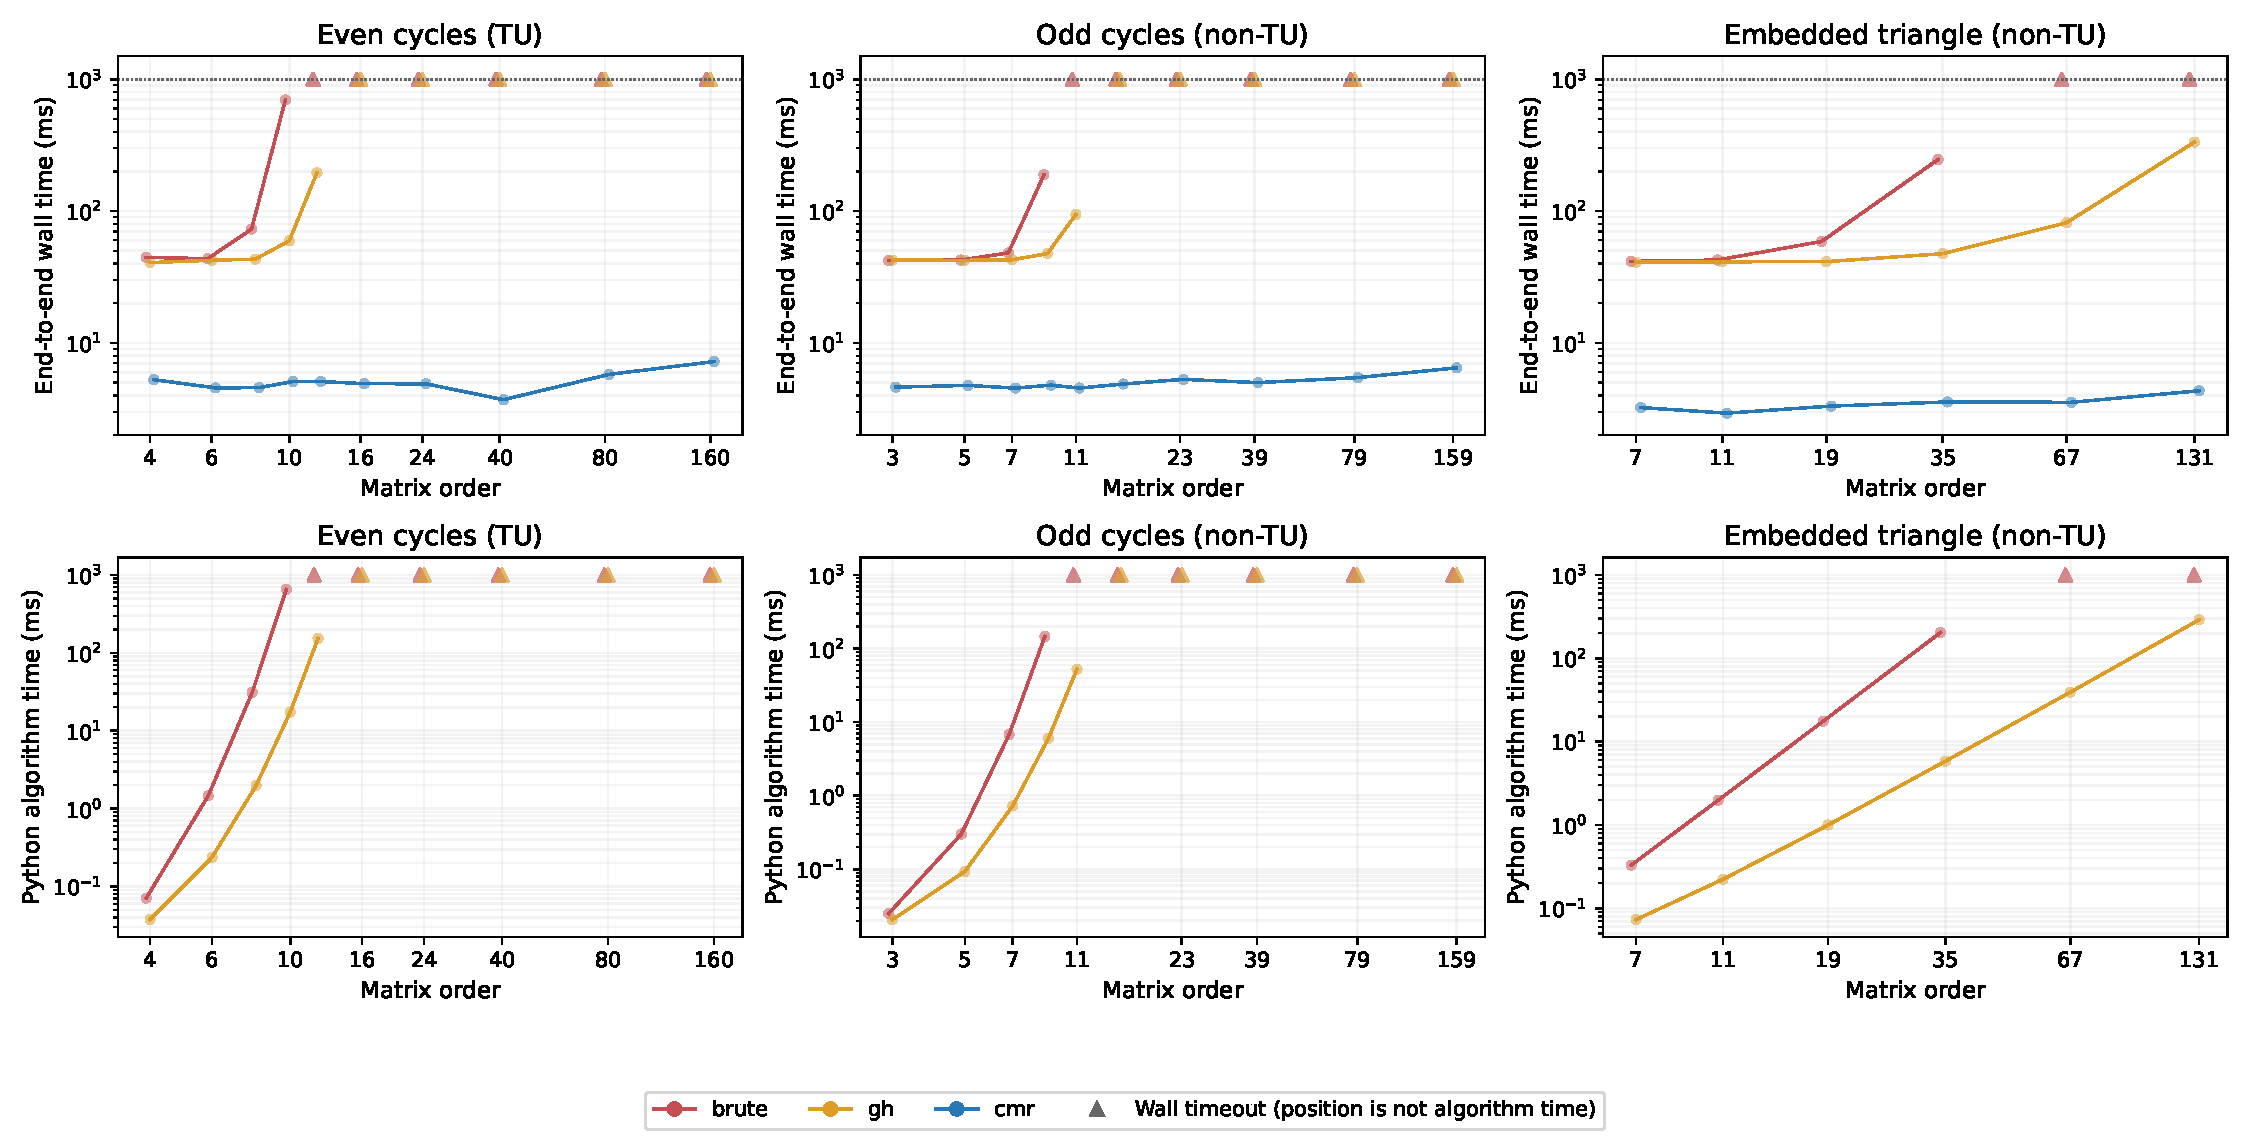
\includegraphics[width=\linewidth,height=0.78\textheight,keepaspectratio]{figures/e2-scaling.pdf}
  \caption{E2 scaling on cycles and the embedded triangle (from \texttt{experiments/E2/analysis}). Top row: end-to-end wall time for all three methods. Bottom row: algorithm time for brute force and GH, without Python start-up; CMR has no comparable internal time. Triangles mark one-second timeouts; their height is not a measured time. Figures for the other families are in the repository.}
  \label{fig:e2}
\end{figure}
\end{landscape}
